
The two temperature-dependent elements of the thermoelectric model---the
radiation-induced digital current increase in the front-end chips, and the
efficiency of the FEAST DC-DC converter---are described in this section.
Both effects are studied experimentally and fit with functional forms
in order to accurately represent them in the model.
The uncertainty in the experimental data, and in our modeling assumptions,
are estimated here and considered in the evaluation of safety factors,
described in detail in Section~\ref{sec:safety_factors}.

\subsubsection{DC-DC converter}

The DC-DC converter (FEAST) supplies a low-voltage (1.5~V) current to the ABC130 and HCC front-end
chips on the module.
The efficiency of the FEAST depends on its temperature as well as the output (load) current
load delivered to the front-end chips. To correctly model the FEAST efficiency, experimental
measurements have been performed to characterize the dependence and fitted with a functional form.

To measure the FEAST efficiency, the FEAST power board was glued to an aluminum cold plate, cooled
with CO$_2$, and powered with the nominal working input and output voltages (11~V input, 1.5~V output).
The temperature of the FEAST was measured with an NTC thermistor and PTAT sensor residing on the FEAST,
for a range of load currents up to the maximum design current of 4A\footnote
{
FEAST data spreadsheet: \url{http://project-dcdc.web.cern.ch/project-dcdc/public/Documents/FEASTMod_Datasheet.pdf}.
Cite?
}.

The data was then fit with a function with sufficient parameters to ensure reasonable agreement; the
choice of functional form has no physical interpretation. Figure~\ref{fig:feast_eff} depicts the
FEAST efficiency data and the parameterized fit used in the model. The parameterization fits the data
with an accuracy below 1\%; this uncertainty in the FEAST efficiency modeling is small
compared to other uncertainty sources, and is therefore neglected in our model.

\begin{figure}[ht]
\centering
\subfloat[] {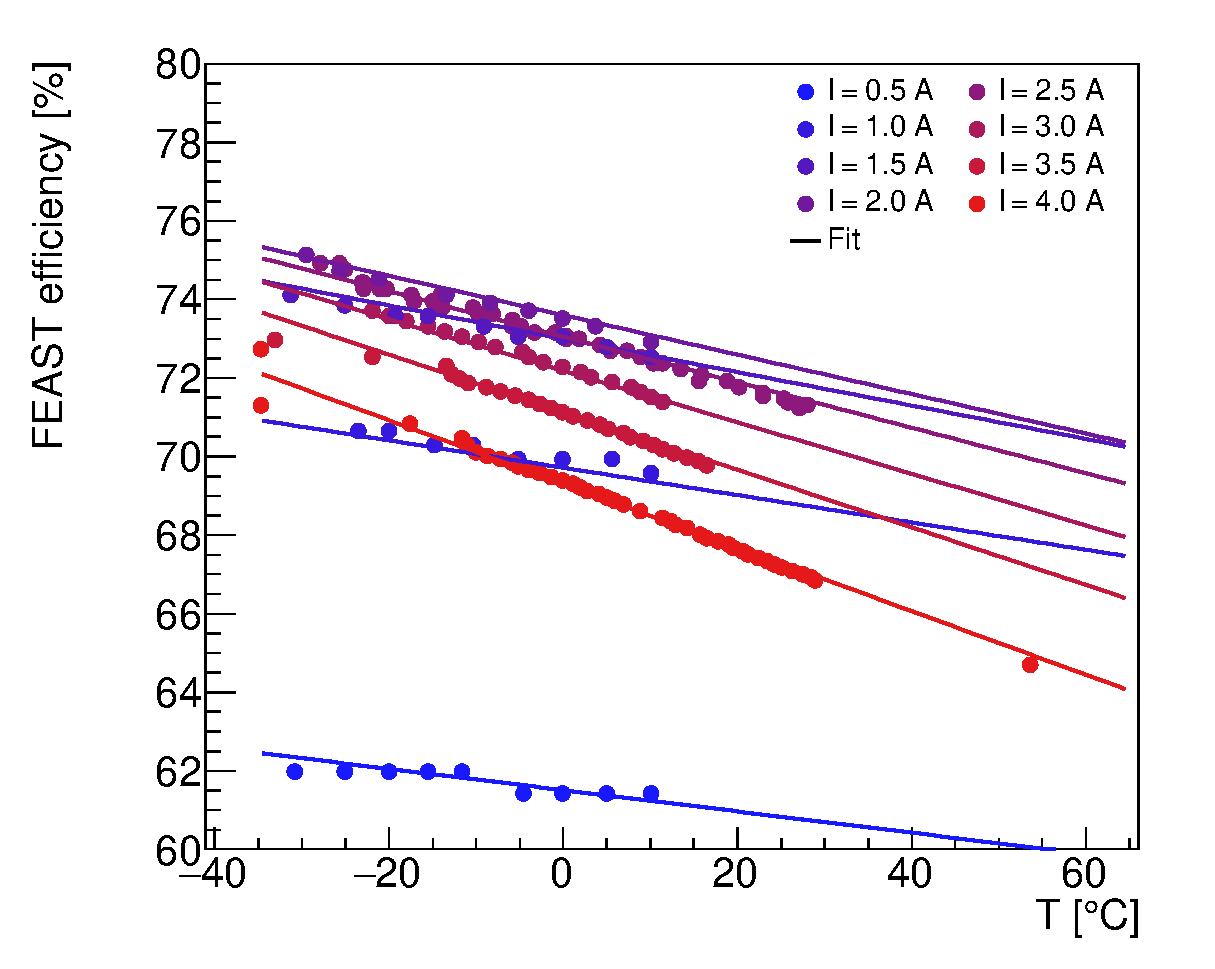
\includegraphics[width=0.45\linewidth]{figures/FeastEfficiency_isoCurrent.eps}}\quad\quad
\subfloat[] {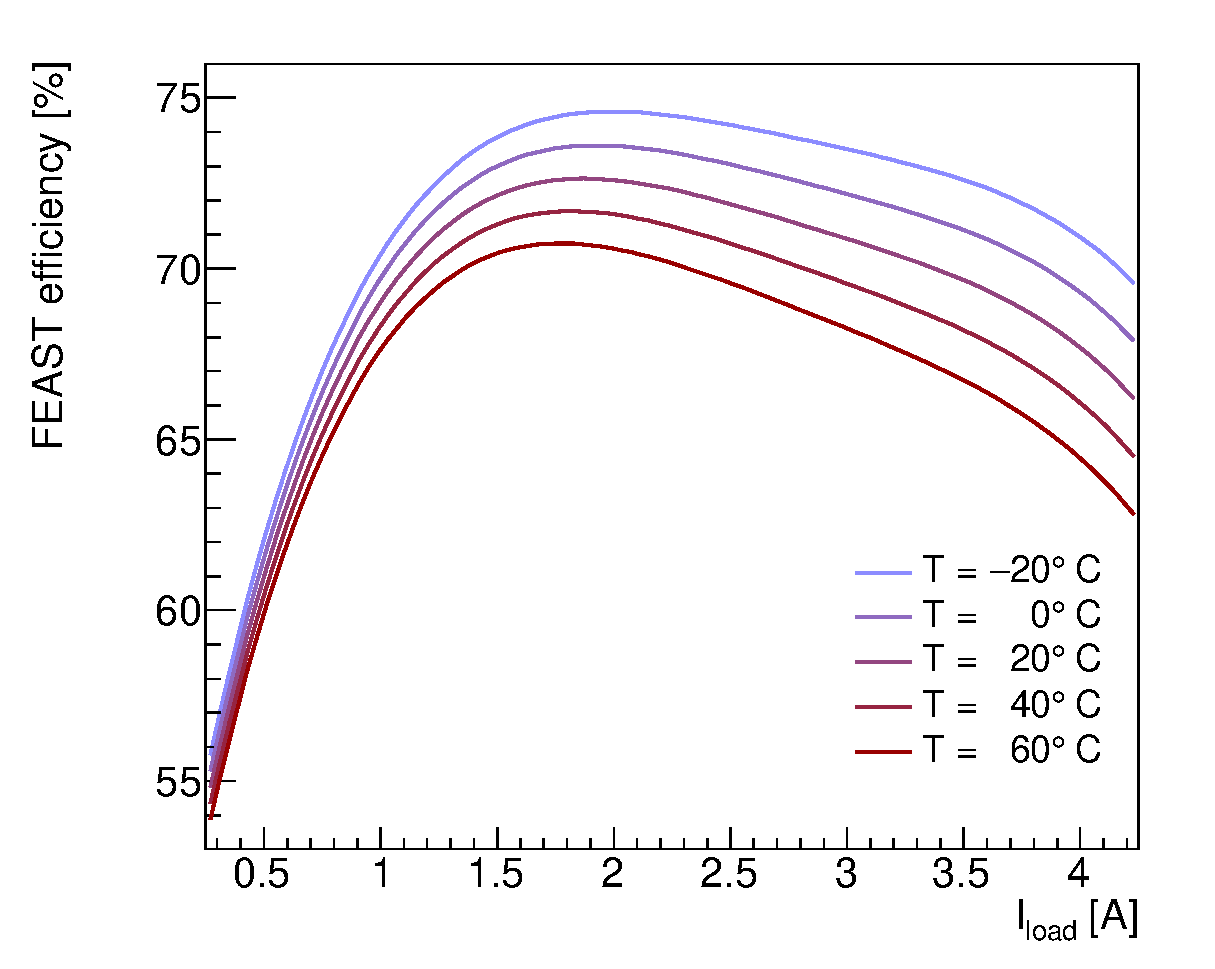
\includegraphics[width=0.45\linewidth]{figures/FeastEfficiency.eps}}
\caption{The FEAST efficiency model based on experimental data. (a) The experimental data points
characterizing the FEAST efficiency are plotted as dots and color coded for load current. The data is
compared to the analytic fit, evaluated in curves of equal current. (b) The same analytic fit,
presented as a function of current load for curves of equal temperature.
}
\label{fig:feast_eff}
\end{figure}


\subsubsection{Digital current increase of chips using 130~nm CMOS technology}
\label{sec:tid_explanation}

The ABC and HCC chips, designed using IBM 130 nm CMOS 8RF technology, are known to suffer from an
increase in digital current when subjected to a high-radiation environment
\cite{Collaboration:2017mtb}. This phenomenon, known as the ``TID bump,'' is well-studied
\cite{1589217,FACCIO20081000} and has a characteristic shape whereby the effect reaches a maximum
as a function of the accumulated dose and then gradually diminishes (see Fig.~\ref{tid_bump}).

\begin{figure}[ht]
\centering
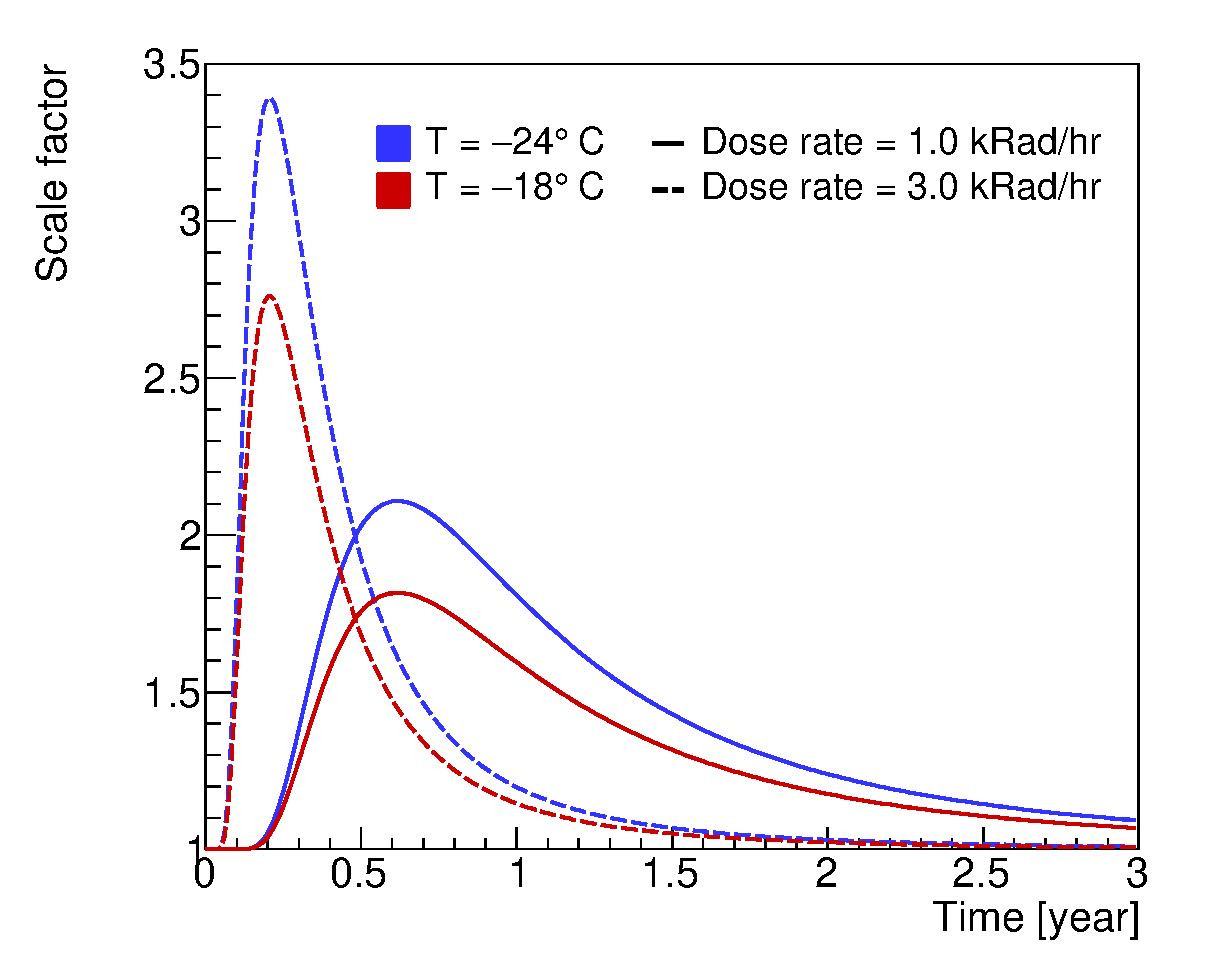
\includegraphics[width=0.45\linewidth]{figures/AbcTidBumpVersionRatesAndTemps_Nominal.eps}
\caption{Parametrization of the impact of the total ionizing dose
on the magnitude of the front-end chip digital current (the TID bump), presented as a function of time.
The current is multiplied by a scale factor that is modeled as a function of total ionizing dose,
dose rate, and temperature, based on experimental data.
}
\label{tid_bump}
\end{figure}

In an effort to characterize the nature of the TID bump in the ABC and HCC chips empirically,
many irradiation campaigns have been conducted using a variety of radiation sources, testing
the effect at different temperatures and dose rates.
The data collected from these studies was used to develop a model of the TID bump
that estimates the digital current increase given the total ionizing dose, the dose rate,
and the operating temperature of the chip. This parameterization, which is depicted in
Fig~\ref{tid_bump}, is used as an input to the thermoelectric model in order to correctly model the
ABC and HCC currents. The TID bump is assumed to fully apply to the HCC digital current, and apply to
69\% of the ABC digital current (according to our understanding of its digital circuitry).

The TID bump displays certain key features, which are reflected in the parameterization:
first, the effect is larger at colder temperatures and higher dose rates. This means it can be
mitigated by operating the chips at higher temperature (note that the dose rate is fixed by the LHC conditions).
Second, the figure also illustrates how chips receiving different dose rates will reach their maximum
digital current increase at different times. This feature is particularly important when modeling the
total power consumed by the barrel and endcap systems. In both systems, the dose rate varies significantly
depending on the position of the module in the detector. The effect means that the maximum system
power will be smaller than the sum of the maximum power of each module, as each chip reaches
its maximum at a different point in time.

The TID bump is an important source of uncertainty in our model. The experimental data suggests
a relatively large variation in the TID bump effect, in particular
between different batches of the same type of chip delivered by the manufacturer, suggesting an unknown
effect in the fabrication process. To estimate the uncertainty in the TID bump,
the parameterized function is fit again using only the worst-performing data (defined as having the
largest TID bump effect). This ``pessimistic'' parameterization is used as a safety factor to estimate
the detector performance in worst-case scenarios.

The irradiations of individual chips have typically been performed at constant dose rate and temperature.
However, both of these parameters will vary as a function of time in the scenarios that we attempt to model.
In our current parametrization, we use only the instantaneous value of these two parameters, thus neglecting any possible history of the TID effect. We also ignore any short-term effects due to variations in the dose rate on the scale of hours or days. This approach is mandated by the lack of more varied experimental data and the absence of a good theoretical model for this effect. This probably constitutes the largest source of unknown error for our model.

\subsubsection{Radiation-dependent leakage current}

The radiation-induced leakage current can be parametrized as a function of the hadron fluence expressed in 1~MeV equivalent neutrons. The parametrizations we have used for the evaluation of our model are shown in Fig.~\ref{fig:leakage} for a reference sensor temperature of $-15^\circ$C. In our model, the leakage current is scaled to a given sensor temperature using Eq.~\ref{eq:leakage_current_temp_dependence}.

\begin{figure}[ht]
\centering
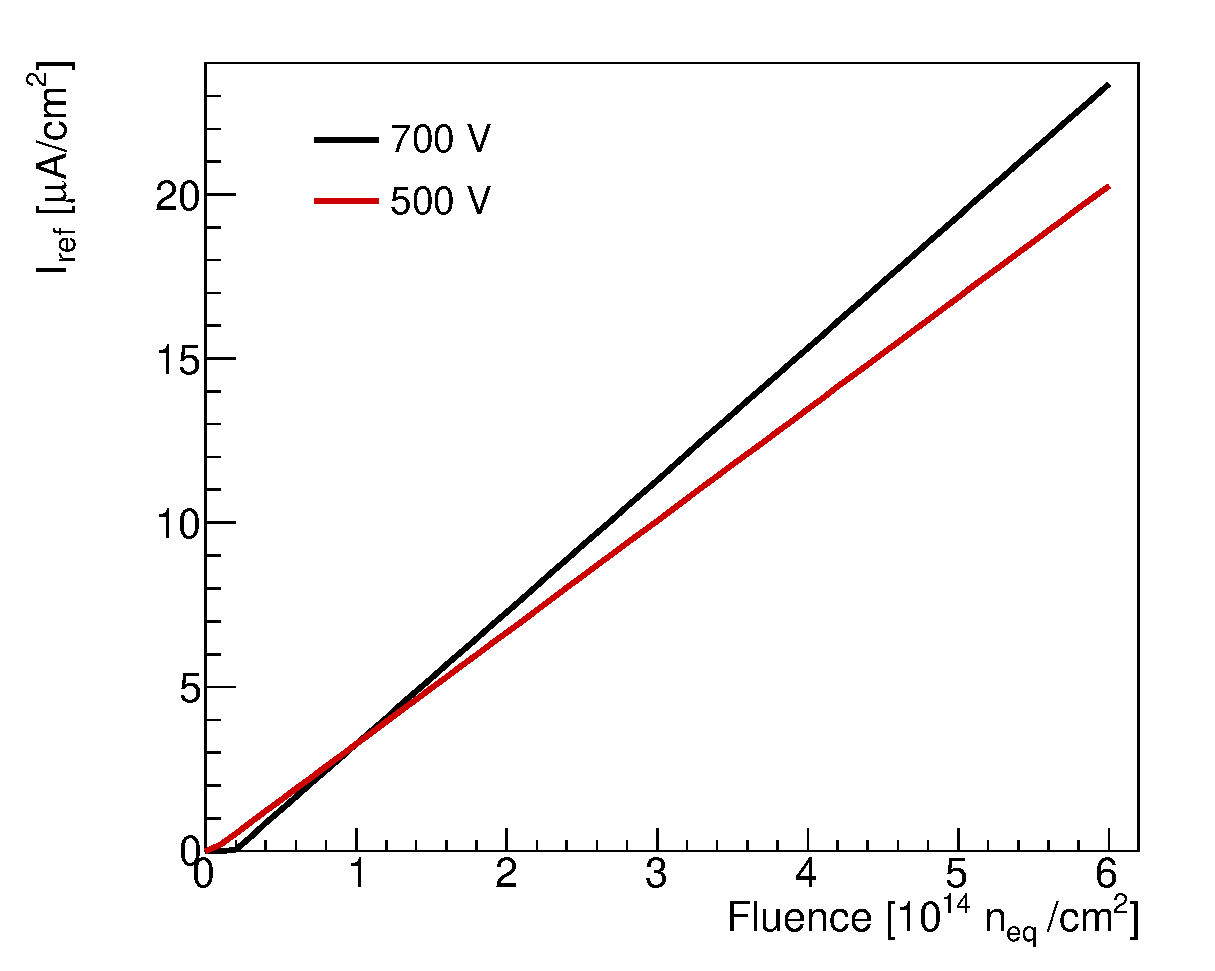
\includegraphics[width=0.45\linewidth]{figures/SensorLeakagePower.eps}
\caption{Parametrization used for the leakage current at $-15^\circ$C as a function of the fluence for two different sensor bias voltages \cite{mikestikova}.}
\label{fig:leakage}
\end{figure}
